% ----------------------------------------------------------
% Fundamentação
% ----------------------------------------------------------
\chapter[Fundamentação Teórica]{Fundamentação Teórica}\label{chap:fundamentacao}

Para que seja possível uma completa compreensão do trabalho e de como usar o sistema por qualquer leitor, independentemente do nível de conhecimento sobre os principais tópicos do trabalho, é feita uma breve definição e elucidação destes tópicos nesse capítulo. Todos os conceitos descritos aqui assumem um prévio conhecimento do que é a Internet e a \textit{World Wide Web}.

\section{Arquitetura Cliente-Servidor}

Estilo de arquitetura criada para resolver o problema de distribuição de recursos. É uma estrutura onde existem dois tipos de participantes: o Cliente e Servidor, ambos denominados processos \cite{tanenbaum2002} dentro da arquitetura. 
 
Servidores são computadores (geralmente de alta performance) designados para atender requisições feitas através da Internet por clientes e também por outros servidores. Ao receber a requisição, o servidor é responsável por executar todo o trabalho solicitado ou retornar dados que o cliente necessita. É um componente que provê um serviço, uma função ou um recurso para o cliente.
 
Cliente e Servidor comunicam-se através de requisição e resposta. O Cliente emite uma requisição através de um protocolo de comunicação (por exemplo, protocolo HTTP) e o Servidor retorna uma resposta pelo mesmo caminho.
 
Existem diversos tipos de servidor, como por exemplo:
\begin{itemize}
	\item Servidor Web, responsável por servir arquivos estáticos ao cliente, carregando os mesmos de um disco rígido, geralmente através do protocolo HTTP.
    \item Servidor FTP, tem como responsabilidade transmitir arquivos ao cliente de maneira segura e sem corromper o arquivo.
    \item Servidor de E-mail, responsável por transmitir e guardar e-mails, utiliza o protocolo SMTP.
    \item Servidor Proxy, peça importante na distribuição de recursos, fica entre o Cliente e um outro Servidor (geralmente Web) e filtra requisições, melhora a performance e escolhe o melhor servidor para o cliente se conectar.
\end{itemize}
 
Essa arquitetura é uma peça importante pois elimina a necessidade do processamento de dados ser feito no computador do cliente \cite{clientserver1996}, possibilitando o uso e acesso de recursos por dispositivos de baixa performance.

\section{Arquitetura Peer-to-Peer}

Estilo de arquitetura que possui somente um tipo de entidade, essa definida de \textit{Servent} por \cite[Sec.~2]{p2pdefinition2001}. \textit{Servent} vem da junção das palavras \textit{Server} e \textit{Client}, indicando que cada \textit{peer} age como um cliente e um servidor. Dito isso, essa arquitetura permite que nodos heterogêneos e distintos possam comunicar-se entre si sem a necessidade de um servidor \cite{p2pgnutella2001}. 
 
Podemos ver pela Figura \ref{fig:clientserver_p2p} que a grande diferença dessa arquitetura para a cliente-servidor, é que a última possuí uma entidade de grande processamento, que possui todos os recursos e todos os nodos se conectam a ele, que é o Servidor.

\begin{figure}[ht!]
	\centering
		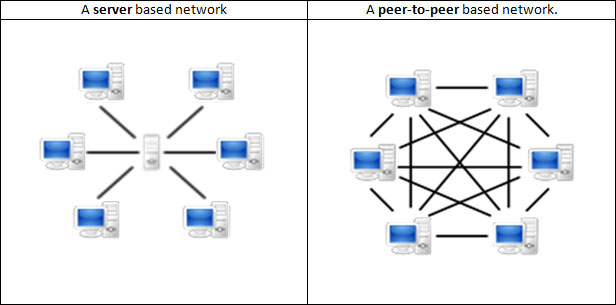
\includegraphics[scale=0.35]{figures/p2p-networks.jpg} 
	\caption{Arquiteturas de rede}
	\label{fig:clientserver_p2p}
\end{figure}

% Citando novamente \cite{p2pdefinition2001}, ele define dois tipos de arquitetura \textit{peer-to-peer}: a híbrida e a pura. A híbrida diz respeito à rede que possui uma entidade central (apesar de ser somente um nodo), a aplicação por trás da estrutura da rede dá a essa entidade mais "poderes" (estilo administrador). A pura como foi citada anteriormente é aquele que é formada somente por \textit{Servents}.
%FRANK: Essa categorização não me parece correta. Procure uma boa referência para isso. O parágrafo inteiro pode ser removido, se não for importante para o trabalho.
%LUCAS: A referencia esta nesse aqui {A definition of peer-to-peer networking}, mas acredito que não seja muito importante para o trabalho.

Podemos dizer então que uma arquitetura distribuída pode ser chamada de \textit{peer-to-peer} se cada um dos seus participantes compartilhar parte dos seus recursos, seja processamento,  armazenamento, banda larga. O que define quais recursos são, é o tipo de rede que está utilizando a arquitetura. 

\section{Arquitetura REST}

\textit{Representational State Transfer} (REST) é um estilo de arquitetura dedicado a sistemas distribuídos, que utiliza \textit{RESTful web services} (serviços Web compatíveis com REST) para facilitar a interoperabilidade de sistemas dentro de uma rede, como a Internet. O termo surgiu pela primeira vez no ano 2000 em uma dissertação de Roy Fielding, um dos principais autores da especificação HTTP.

De acordo com \cite{restroyfielding2000} a lógica por trás de uma arquitetura para \textit{Web} é descrita por um conjunto de restrições aplicadas aos elementos da arquitetura.

REST, utiliza padrões e restrições para definir como recursos da Internet devem ser definidos e utilizados. Algumas das restrições são:
\begin{itemize}
	\item Utilizar arquitetura cliente-servidor.
	\item Toda operação é \textit{stateless}, ou seja, não guarda estado; cada requisição ao servidor deve conter toda informação necessária para realizar a operação.
	\item O sistema deve implementar uma camada de \textit{cache} para melhorar a eficiência na rede (devido à natureza \textit{stateless}).
\end{itemize}

Interoperabilidade entre sistemas, significa acima de tudo a possibilidade de troca de informações dentro da arquitetura. Observamos na tabela \ref{table:elemento-de-dados-rest} a definição de elementos de dados que especificam o tipo de informação disponível e como chegar até ela.

\begin{table}[ht!]
	\centering
	\begin{tabular}{@{}ll@{}}
		\toprule
		\textbf{Elemento de dados}       & \textbf{Exemplos da web}       \\ \midrule
		\textit{resource}                & Mapeamento conceitual de uma referência em hipertexto   \\
		\textit{resource identifier}     & URL, URN, URI                                      \\
		\textit{representation}          & Documento HTML, imagem JPEG                        \\
		\textit{representation metadata} & Tipo de mídia, última data de modificação          \\
		\textit{resource metadata}       & Fonte do link    \\
		\textit{control data}            & if-modified-since, cache control (cabeçalhos HTTP) \\ 
        \bottomrule
	\end{tabular}
	\caption{Elementos de dados REST}
    \label{table:elemento-de-dados-rest}
\end{table}

O conceito chave de informação no REST é \textit{resource}. Esse pode ser um texto, uma imagem, um serviço, dentre outros. Para identificar um recurso específico no servidor utiliza-se identificadores de recursos (\textit{resource identifiers}), usualmente conhecidos como \textit{link} ou URL. 

Ao acessar um identificador recebemos uma representação (\textit{representation}) que remete ao estado (\textit{state}) do recurso em determinado momento no tempo. 
%FRANK: rever a última frase
%LUCAS: Revi e fiz mais alterações. Por favor reveja 26/11
%FRANK: Cortei o que achei desnecessário e confuso. (27/11)

REST geralmente é implementado por servidores sobre o protocolo de comunicação HTTP utilizando os mesmos verbos disponíveis (GET, POST, PUT, DELETE) no protocolo. No servidor é definido um conjunto de "operações sem estado" e através dessas operações os servidores tem acesso aos chamados \text{Web resources}.

Existem outros serviços da Web que fornecem interoperabilidade e a noção de recursos, porém com suas próprias características, como por exemplo, WSDL e SOAP.

Esse estilo de arquitetura foi escolhido para o trabalho por ser o mais difundido na comunidade hoje em dia. No sistema de atendimento ao consumidor será utilizada a arquitetura REST em um servidor API com o objetivo de salvar as interações dos usuários com o nosso sistema (chamadas de vídeo, requisições de atendimento, dentre outras).

\section{Protocolo HTTP}

\textit{HyperText Transfer Protocol} (em português protocolo de transferência de hipertexto) é um protocolo utilizado em nível de aplicação em modelos como o TCP/IP. Serve principalmente para transferir informações em sistemas distribuídos como a \textit{World Wide Web}, provavelmente o mais popular.

Dentro de um sistema massivo de informação como a Internet o protocolo HTTP funciona através de operações requisição-resposta sem estado. De acordo com \cite[Sec.~4]{httprfc2616} essas operações são mensagens de texto que obedecem a um padrão definido pela especificação HTTP.

Existem duas entidades principais em uma mensagem HTTP. O cliente que envia uma mensagem requisitando um recurso, e o servidor que a processa e responde de acordo com os dados da requisição.

A mensagem de requisição deve especificar um método dentre um conjunto definido pelo protocolo de transferência. Conforme \cite[Sec.~9]{httprfc2616}, cada método do protocolo determina o tipo de operação feita no servidor e o resultado a ser esperado. A Tabela \ref{table:metodos-http} descreve os principais métodos definidos na especificação do protocolo.

\begin{table}[ht!]
	\centering
	\begin{tabular}{@{}ll@{}}
		\toprule
		\textbf{Método}	     & \textbf{Descrição}       \\ \midrule
		GET		             & Retorna dados de um recurso específico.       \\
		DELETE			     & Remove um recurso específico.         \\
		POST          	  	 & Modifica ou altera um recurso. Não cria.     \\
        PUT          	  	 & Cria ou sobrescreve um recurso.     \\
		OPTIONS				 & Lista as opções de comunicação com o recurso.         \\
        \bottomrule
	\end{tabular}
	\caption{Métodos HTTP}
    \label{table:metodos-http}
\end{table}
%FRANK: faltou PUT
%LUCAS: pronto

A responsabilidade do servidor é responder com o código de estado e o recurso requerido, se existente. Observamos em \cite[Sec.~10]{httprfc2616} que o código de status faz parte de um conjunto de números que refletem o resultado da requisição. Consulte a Tabela \ref{table:codigos-http}, na qual encontram-se os códigos mais usados e o seu significado.

\begin{table}[ht!]
	\centering
	\begin{tabular}{@{}ll@{}}
		\toprule
		\textbf{Código de estado}	     & \textbf{Significado}       \\ \midrule
		200		             & Requisição bem sucedida.       \\
		301				     & Recurso movido permanentemente.         \\
		404          	  	 & Recurso não encontrado.                      \\
		500				     & Erro no servidor.         \\
        \bottomrule
	\end{tabular}
	\caption{Códigos HTTP}
    \label{table:codigos-http}
\end{table}


Fundamental em toda aplicação que deseja buscar ou enviar informações através da Internet, pode ser usado como base para outros tipos de protocolo, como o protocolo \textit{WebSocket} que será abordado no próximo capítulo, ou também para arquiteturas como REST, abordada na seção anterior. 

\section{Protocolo WebSocket}

Com o avanço da Internet, surgiram novos tipos de aplicações como alternativa ao paradigma usual de requisição-resposta.
A Internet tornou-se uma plataforma onde enviamos todo tipo de dado para comunicação entre computadores. O surgimento de jogos online, programas de mensagem instantânea e aplicações em tempo real de modo geral, mostrou que é necessário avançar além da versão 1.0 do protocolo HTTP.
Algumas estratégias foram criadas para mitigar esse problemas, uma delas chamada \textit{long polling}. Nessa técnica após a primeira requisição o servidor mantém a conexão TCP aberta até ter novos dados para enviar ao cliente. Quando o cliente recebe os novos dados, automaticamente realiza uma nova solicitação.
Usar esse tipo de técnica traz algumas desvantagens, de acordo com \cite[Sec.~1]{websocketprotocol2011}:

\begin{itemize}
	\item Repetidas conexões TCP.
    \item Sobrecarga na conexão por ter que enviar cabeçalhos HTTP para cada mensagem trocada entre cliente e servidor.
    \item A nível de código é necessário implementar um gerenciador de requisições e respostas.
\end{itemize}

Como solução foi proposto o protocolo WebSocket, que utiliza somente uma conexão TCP bidirecional, sem sobrecarga de requisições, para comunicação entre as duas partes.

O WebSocket funciona em cima de conexões TCP, propositalmente para que seja compatível com servidores antigos que ainda não suportam o novo protocolo, e envolve duas partes, abertura de conexão e transferência de dados.
A primeira é uma requisição HTTP feita pelo cliente indicando (através de cabeçalhos) que quer atualizar a conexão para WebSocket. Caso o servidor entenda o protocolo, concordará em fazer a troca. Esse processo todo foi nomeado WebSocket \textit{handshake}.

Com o \textit{handshake} aceito, a conexão está estabelecida e agora existe um canal bidirecional entre cliente e servidor, pela qual cada parte pode enviar e receber dados a qualquer momento. Cada unidade de dados transferida é chamada de mensagem ou \textit{frame} (a nível de cabeamento).

%FRANK: como assim? rever essa expressão
%LUCAS: 26/11
% REMOVI -  protocolo não seja explicitamente usado na aplicação, ele é utilizado por debaixo dos panos 
% ADICIONEI - O protocolo é utilizado de forma subjacente na aplicação
O protocolo é utilizado de forma subjacente na aplicação pelo \textit{framework} Socket.IO (abordada no capítulo de projetos). Essa tecnologia facilita a implementação do servidor responsável pelo processo de \textit{signaling} (em português, sinalização), que é similar ao \textit{handshake} e necessário para realizar conexões ponto-a-ponto através do WebRTC. 

\section{WebRTC}

Desde a criação da World Wide Web, seu objetivo foi sempre o de permitir o acesso a informações de forma fácil e rápida. No primeiro momento textos com \textit{hyperlinks} levavam a outros textos, e depois a imagens, áudios, vídeos, ou seja, todo tipo de mídia capaz de ser reproduzida digitalmente. Porém, todos representados estaticamente.

Um dos maiores desafios da Web hoje em dia é a comunicação por vídeo e voz em tempo real, \textit{Real Time Communication} ou RTC. 
A mudança veio junto do lançamento do Google Chat em 2008, que permitiu a seus usuários conversarem olhando um para o outro através de seus navegadores. 

Buscando o avanço da tecnologia, a Google disponibilizou os \textit{codecs} de áudio e vídeo e outras técnicas utilizadas para comunicação em tempo real e criou grupos de pessoas responsáveis por padronizar e aprimorá-los criando especificações. Finalmente, em 2011 a Ericsson surgiu com a primeira implementação do WebRTC (\cite{ericssonwebrtc}).

A tecnologia WebRTC é composta de um conjunto de especificações criadas por grupos de pessoas de instituições como W3C e IETF, além de empresas fabricantes de navegadores. Esses documentos têm como objetivo padronizar interfaces que serão responsáveis por realizar chamadas em tempo real, e os fabricantes de navegadores ficam com a responsabilidade de implementá-las em seus produtos. Com isso, busca-se permitir a comunicação entre usuários que utilizam diferentes \textit{browsers}. 

Atualmente as principais especificações envolvem três interfaces de programação de aplicações, que serão detalhadas nas próximas seções:

\begin{itemize}
	\item MediaStream (ou getUserMedia) \cite[Sec.~4.2]{getusermedia2017}
    \item RTCPeerConnection \cite[Sec.~4.4]{w3cwebrtc2017}
    \item RTCDataChannel \cite[Sec.~4.6]{w3cwebrtc2017}
\end{itemize}

\subsection{MediaStream}

Interface responsável por consumir fontes de áudio e vídeo em forma de fluxo de dados e controlar para onde esse fluxo vai ser direcionado -- por exemplo, uma saída de áudio, elemento HTML, dentre outros.  A especificação também define funções que fornecem acesso a dispositivos de mídia, como câmeras e microfones, de acordo com as permissões do usuário. 

Com o acesso permitido, as informações chegam como \textit{streams} (fluxos) de mídia e são conectadas ao \textit{input} de um objeto MediaStream. Esse objeto possui múltiplas trilhas (\textit{tracks}) e cada uma delas corresponde a um tipo diferente de mídia (vídeo de uma câmera, música de um mp3, etc.). 

\begin{figure}[ht!]
	\centering
		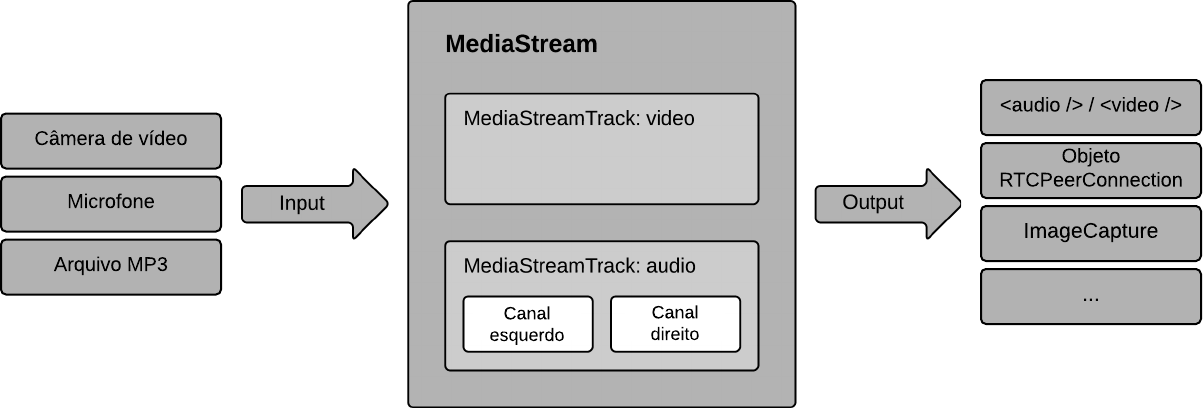
\includegraphics[scale=0.35]{figures/overview-mediastream.png} 
	\caption{Fluxo de dados usando MediaStream}
	\label{fig:overview_mediastream}
\end{figure}

Os chamados consumidores de MediaStream são objetos que conseguem ler o fluxo de dados do \textit{output} dessa interface. A imagem \ref{fig:overview_mediastream} mostra exemplos de saídas existentes. A maior vantagem para o WebRTC é o fluxo poder ser enviado através de objetos RTCPeerConnection, sendo transportado como \textit{streams}, permitindo assim chamadas de áudio e vídeo remotas. Os elementos HTML de áudio e vídeo são responsáveis pela reprodução de mídias no cliente e aceitam saídas MediaStream como entradas de dados.

\subsection{RTCPeerConnection}

De acordo com \cite[Sec.~4.1]{w3cwebrtc2017} é possível realizar conexões ponto-a-ponto entre diferentes computadores em uma rede através de dois objetos RTCPeerConnection. A conexão é realizada através de uma troca de mensagens padronizada por um protocolo de sinalização, similar ao \textit{handshake} do TCP, porém no nível de aplicação. 

Essa troca é chamada de \textit{signaling} e não está definida na especificação, cabendo ao desenvolvedor escolher a maneira de realizá-la. Geralmente é utilizado um servidor que funciona através de WebSockets (no caso desse projeto), requisições HTTP, dentre outros mecanismos.

Em projetos WebRTC executados em uma única aba no navegador não é necessário o uso de um servidor, as informações estão no mesmo contexto de código e conseguimos realizar a conexão sem troca de mensagens através da Internet. Quando alteramos a aplicação para o âmbito da Web, funcionando em produção com \text{peers} remotos, basicamente precisamos de quatro funcionalidades no lado dos servidores:

\begin{itemize}
	\item Tradução de endereço local para público;
    \item Descobrir endereço de IP público do próprio usuário (não do *peer* remoto);
    \item Retransmissão de dados através de servidor reserva caso a conexão ponto-a-ponto não funcione, ou não seja suportada;
    \item Sinalização do cliente enviada para o remoto indicando conexão P2P.
\end{itemize}

Todos esses pontos, exceto o da sinalização, são resolvidos por um protocolo chamado \textit{Interactive Connectivity Establishment} (ICE), que geralmente é utilizado por aplicações WebRTC.

\begin{figure}[ht!]
	\centering
		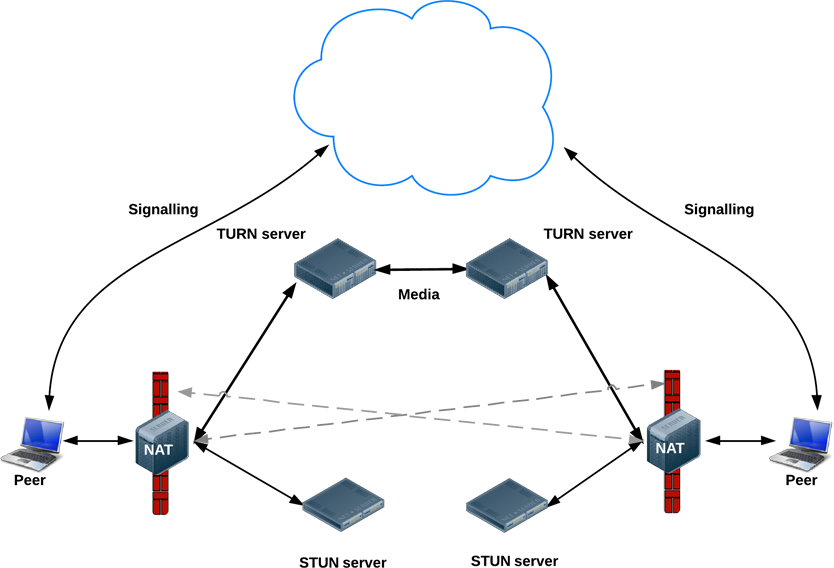
\includegraphics[scale=0.35]{figures/overview-iceprotocol.png} 
	\caption{Protocolo ICE, retirado de \cite{webrtcarchitecture}}
	\label{fig:overview_iceprotocol}
\end{figure}

A figura \ref{fig:overview_iceprotocol} apresenta uma visão geral do processo de \textit{signaling} e seus componentes principais, que são responsáveis cada um por uma  funcionalidade citada acima:

\begin{itemize}
	\item NAT - Responsável por gerar um endereço IP público através de uma tabela \textit{hash} para o cliente;
    \item STUN - Servidor público ou privado, responde com endereço de IP gerado pelo NAT através de uma requisição feita pelo mesmo cliente;
    \item TURN - Servidor responsável por retransmitir os dados caso a conexão ponto-a-ponto não funcione.
\end{itemize}

Com a conexão \textit{peer-to-peer} estabelecida, o servidor deixa de ser necessário e os navegadores estão aptos a transmitir informações em tempo real.

\subsection{RTCDataChannel}

Além de enviar áudio e vídeo, WebRTC tem a capacidade de se comunicar em tempo real por meio da interface RTCDataChannel  usando diversos tipos de dados. 

Essa funcionalidade foi implementada devido a certos casos de uso, como jogos online, transferência de arquivos, documentos de textos colaborativos (por exemplo, Google Docs), dentre outros.

O objetivo é atingir uma baixa latência aliada a uma alta capacidade de transmissão de dados, devido à redução de sobrecarga por \textit{handshakes} TCP e cabeçalhos HTTP. É utilizado o mesmo tipo de conexão para fluxos de áudio e vídeo, através de um objeto RTCPeerConnection. Apesar de muito similar a conexões WebSockets, é mais rápida devido ao fato de estabelecer uma conexão direta de um navegador a outro.

WebRTC é a fundação do sistema de atendimento implementado nesse projeto. A capacidade de comunicação em tempo real, utilização diretamente do navegador e a não necessidade de instalar \textit{plugins} de terceiros, tornaram a ferramenta ideal para solucionar os problemas apresentados no início do trabalho.

